\begin{frame}[fragile,t]
  \frametitle{From Taylor-mode to Forward Laplacian}

  \vspace{-2ex}
  \emph{Example:} Laplacian \quad $\Delta f_i^{(L)}(\vx) = \sum_j \frac{\partial^2 f_i^{(L)}(\vx)}{\partial x_j^2} = \sum_j \partial^2_{\ve_j} f_i^{(L)}(\vx)$
  \vspace{-2ex}

  \begin{figure}[t]
    \centering
    \hspace*{-3ex}
    \begin{tikzpicture}
      \matrix (magic)
      [matrix of nodes,
      ampersand replacement=\&,
      nodes={
        anchor=center,
        inner sep=2pt,
      }]
      {
        $f^{(0)} = \operatorname{id}$
        \& $f^{(1)} \circ f^{(0)}$
        \& $\dots$
        \& $f^{(L)} \circ \ldots \circ f^{(0)}$
        \\
        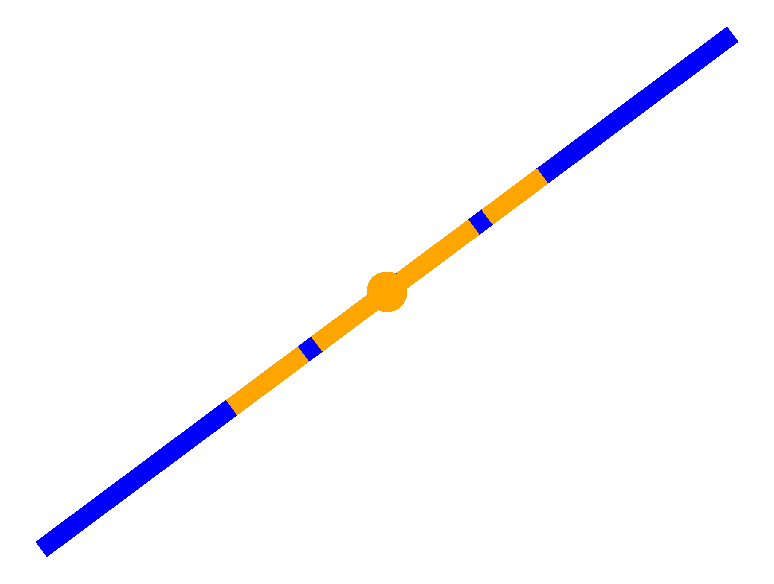
\includegraphics[scale=0.23]{/Users/fdangel/Documents/Postdoc/kfac-pinns/kfac_pinns_exp/exp48_visualization_taylor_mode/f_0_taylor_2.pdf}
        \& 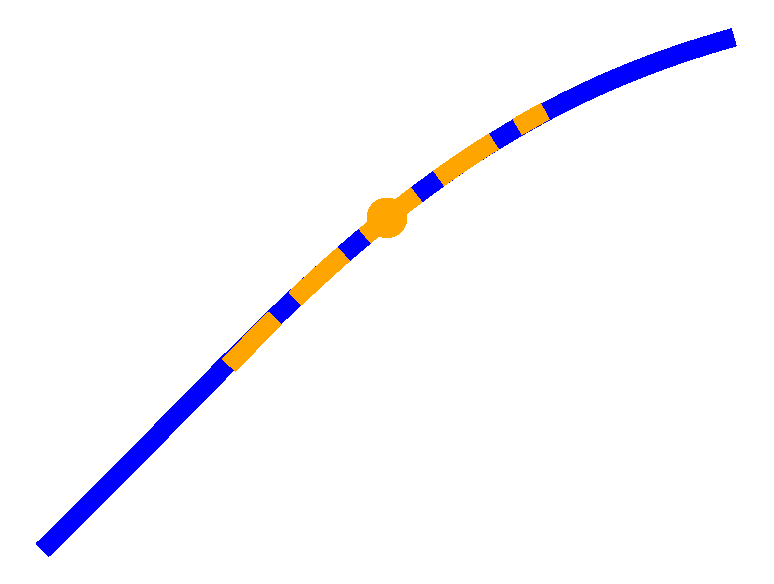
\includegraphics[scale=0.23]{/Users/fdangel/Documents/Postdoc/kfac-pinns/kfac_pinns_exp/exp48_visualization_taylor_mode/f_1_taylor_2.pdf}
        \& 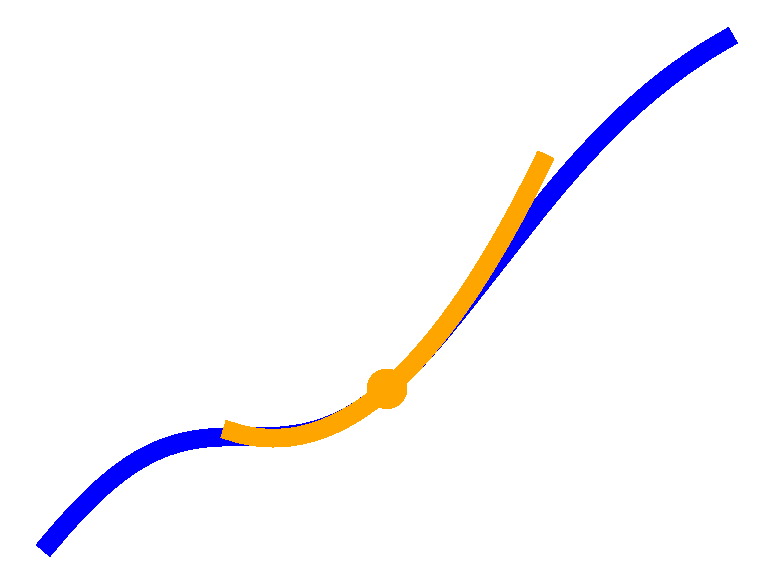
\includegraphics[scale=0.23]{/Users/fdangel/Documents/Postdoc/kfac-pinns/kfac_pinns_exp/exp48_visualization_taylor_mode/f_2_taylor_2.pdf}
        \& 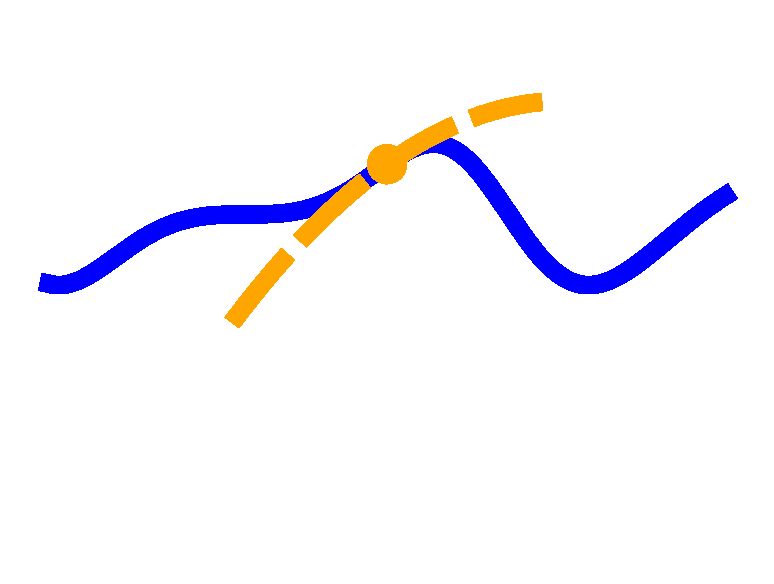
\includegraphics[scale=0.23]{/Users/fdangel/Documents/Postdoc/kfac-pinns/kfac_pinns_exp/exp48_visualization_taylor_mode/f_3_taylor_2.pdf}
        \\
        $f^{(0)}(\vx) = \vx$
        \& $\left\{ f_i^{(1)}(f^{(0)}(\vx)) \right\}_i$
        \&$\dots$
        \&$\left\{ f_i^{(L)}(f^{(L-1)}(\vx)) \right\}_i$
        \\
        $\left\{\partial_{\only<1>{\vv}\only<2->{\ve_j}} f_i^{(0)}(\vx) = v_{i}\right\}_{i\only<2->{,j}}$
        \&$\left\{\partial_{\only<1>{\vv}\only<2->{\ve_j}} f_i^{(1)}(\vx) \right\}_{i\only<2->{,j}}$
        \&$\dots$
        \&$\left\{\partial_{\only<1>{\vv}\only<2->{\ve_j}} f_i^{(L)}(\vx) \right\}_{i\only<2->{,j}}$
        \\
        $\left\{\partial^2_{\only<1>{\vv}\only<2->{\ve_j}} f_i^{(0)}(\vx) = 0 \right\}_{i\only<2->{,j}}$
        \&$\left\{\partial^2_{\only<1>{\vv}\only<2->{\ve_j}} f_i^{(1)}(\vx) \right\}_{i\only<2->{,j}}$
        \&$\dots$
        \&$\left\{\partial^2_{\only<1>{\vv}\only<2->{\ve_j}} f_i^{(L)}(\vx) \right\}_{i\only<2->{,j}}$
        \&\node [align=center] {\textcolor{orange}{\textbf{Na\"ive:}}\\ \textcolor{orange}{$\sum_j \partial^2_{\ve_j} f_i^{(L)}(\vx)$}};
        \\
        \only<3->{
          $\left\{\Delta f_i^{(0)}(\vx) = 0\right\}_i$
          \& $\left\{\Delta f_i^{(1)}(\vx) \right\}_i$
          \&$\dots$
          \& $\left\{\Delta f_i^{(2)}(\vx) \right\}_i$
          \& \node [align=center] {\textcolor{orange}{\textbf{Forward}}\\ \textcolor{orange}{\textbf{Laplacian}}};
        }
      };
    \end{tikzpicture}
  \end{figure}
\end{frame}
%%% Local Variables:
%%% mode: LaTeX
%%% TeX-master: "../pitch"
%%% End:
